\documentclass[11pt,a4paper]{article}
\usepackage[top=1.1in,left=1.15in,right=1.15in,bottom=1in]{geometry}
\usepackage[T1]{fontenc}
\usepackage{lmodern,microtype,amsmath,amssymb,amsthm,booktabs,graphicx,array}
\usepackage{tikz}
\usetikzlibrary{arrows.meta,positioning,fit,calc,shapes.geometric,decorations.pathreplacing}
\usepackage[ruled,linesnumbered]{algorithm2e}
\usepackage[round]{natbib}
\usepackage[hidelinks]{hyperref}
\makeatletter\g@addto@macro\UrlBreaks{\do\_\do\-}\makeatother
\newtheorem{definition}{Definition}
\newtheorem{proposition}{Proposition}
\newcommand{\Prob}{\mathbb P}
\setlength{\emergencystretch}{2em}
\graphicspath{{./}{../}}

\begin{document}
\begin{center}
{\Large\bfseries Deploying attack-conditional disclosure audits at an international financial institution:\\[2pt] a protocol for release governance and penetration testing\par}
\vspace{4mm}
Ronald Rethabile Malamule Mahomane\\[2pt]
{\small Department of Computing, Mathematical and Statistical Sciences, University of Namibia, Windhoek\\
School of Pathology, Faculty of Health Sciences, University of the Witwatersrand, Johannesburg\\
Basis Energy, Victoria, Australia\\
Corresponding author: \href{mailto:ron@basisenergygroup.com}{ron@basisenergygroup.com}}\\[2pt]
{\small Author manuscript, October 2026. Not a BIS or IFC publication.}
\end{center}

\begin{abstract}
Two companion papers set out a method for governing disclosure risk across repeated statistical releases: risk is the measured success of a declared attack, a release is certified when an exact or anytime-valid upper bound on that success falls below a tolerance set by a named owner, a programme spends one error budget across its releases and audits, and every step is written to a keyed, hash-chained ledger. This paper asks how an institution would deploy it. We take the Bank for International Settlements as the case, because its statistical products are built from confidential national data, released in overlapping vintages through a query portal, and in one case shared at the institution level with supervisors. We map the method's requirements onto those programmes and set out roles, phases and a registry service. We then make one addition to the method. A dissemination portal is software, and a software flaw changes what an adversary can see; so a penetration-test finding is a statement about the adversary's information set and belongs in the audit. We give a closed list of capabilities that findings grant, a monotone composition rule, and a protocol under which each confirmed finding becomes an audited adversary with a share of the programme's error budget. A worked example on a public Census extract, with four PHP advisories from 2026 as the findings, shows a release that passes as published, fails under a suppression bypass, passes under a credential leak alone, and fails when the two are pooled. The finding ranked by measured disclosure risk is not the finding ranked highest by its severity score.
\end{abstract}

\section*{Executive summary}
\paragraph{Situation.} The BIS publishes international banking, debt-securities, derivatives, credit and property-price statistics compiled from data that central banks hold in confidence, and it disseminates them through a data portal that lets a user build tables across reporting countries, counterparties, instruments and quarterly vintages. The International Data Hub goes further: institution-level data on large banks are compiled and shared with designated supervisors \citep{bisstats}. Disclosure review of such products is done one release at a time, by rules such as minimum cell counts.

\paragraph{Complication.} Three things break per-release review. Vintages overlap, so an adversary who pools them faces a risk that no per-release figure bounds. The list of attacks grows as audits are read, so a procedure that controls error for a fixed list does not cover the list the institution actually tests. And the portal is a software system: a flaw in it can give the adversary cells the mechanism suppressed, or readings the mechanism blurred, and no cell-count rule accounts for that.

\paragraph{Question.} How does an institution adopt attack-conditional, budgeted, ledgered disclosure audits for live programmes, and how does it bring its security testing into the same accounting?

\paragraph{Answer.} Deploy in three phases, each a programme at a time: a shadow run that measures declared attacks on past releases without gating them; a gated run in which a release committee owns the tolerance and a registry service owns the keys, the clock and the budget; then penetration testing in which every confirmed software finding is declared as a capability, composed into an adversary view, measured with the same executable attacker, and certified or refused at a share of the programme's budget. The worked example shows why this matters: a critical-rated flaw that is not exploitable adds nothing, a high-rated access-control flaw turns a passing release into a failing one, and two individually tolerable flaws fail together.

\section{Introduction}\label{sec:intro}
The method this paper deploys is developed in two companion manuscripts. The long form \citep{mahomane2026long} sets out the probability model: a release is a mechanism applied to a register, an adversary is a declared information set and a matching rule, and the risk of a release is the success probability of that attack, estimated by simulation with its own certification cost. It shows that marginal risks do not bound a pooled attack across releases, derives the tolerance implied by a stated price of harm, and gives an operational protocol with falsification tests. The journal article \citep{mahomane2026adaptive} adds the adaptive part: each pair of a candidate release and a declared attack is a coordinate certified by a test supermartingale, coordinates can be added after outcomes are seen, the programme spends one error budget, and the audit process itself has a threat model with measured attacks and controls. The code that produced both is public \citep{privacyriskcode}.

Neither paper says how an institution would run this. The present paper does, for one institution, and it adds a piece the earlier papers left out. Section \ref{sec:requirements} states what the method needs from an institution. Section \ref{sec:bis} maps those needs onto BIS statistical programmes. Section \ref{sec:software} argues that the software layer of a dissemination system is part of the adversary model and gives the 2026 PHP advisories as a worked list. Section \ref{sec:pentest} sets out the penetration-testing protocol, with Algorithm \ref{alg:pentest} and the worked example in Table \ref{tab:pentest}. Section \ref{sec:deploy} gives the deployment architecture (Figure \ref{fig:architecture}), roles and phases. Section \ref{sec:limits} says what is not claimed.

\section{What the method requires of an institution}\label{sec:requirements}
Figure \ref{fig:method} summarises the method as the institution sees it. Five things must exist before the first gated release.

\begin{figure}[htbp]
\centering
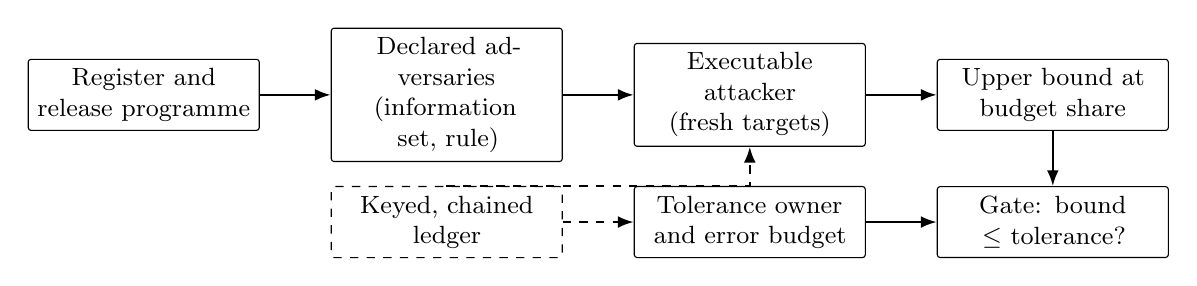
\begin{tikzpicture}[font=\small, node distance=7mm and 9mm,
  box/.style={draw, rounded corners=1pt, minimum height=9mm, text width=27mm, align=center},
  arr/.style={-{Latex[length=2mm]}, thick}]
\node[box] (reg) {Register and\\release programme};
\node[box, right=of reg] (adv) {Declared adversaries\\(information set, rule)};
\node[box, right=of adv] (att) {Executable attacker\\(fresh targets)};
\node[box, right=of att] (bound) {Upper bound at\\budget share};
\node[box, below=of bound] (gate) {Gate: bound\\$\le$ tolerance?};
\node[box, left=of gate] (owner) {Tolerance owner\\and error budget};
\node[box, left=of owner, dashed] (ledger) {Keyed, chained\\ledger};
\draw[arr] (reg) -- (adv); \draw[arr] (adv) -- (att); \draw[arr] (att) -- (bound);
\draw[arr] (bound) -- (gate); \draw[arr] (owner) -- (gate);
\draw[arr, dashed] (ledger) -- (owner);
\draw[arr, dashed] (ledger.north) |- ($(adv.south)+(0,-3mm)$) -| (att.south);
\end{tikzpicture}
\caption{The method as an institution runs it. Solid arrows are the audit of one release; the dashed ledger records every declaration, plan and outcome before and after the fact. The figure uses line style, not colour, to separate the audit path from the record.}
\label{fig:method}
\end{figure}

\begin{enumerate}
\item \emph{Declared adversaries.} Each adversary is an information set and a matching rule, written down before any outcome is read. The long form's credit-register case uses three: an outsider with one release, an outsider who pools vintages and knows when the target was present, and an insider who knows exposure to within a stated error.
\item \emph{An executable attacker.} Risk is measured, not scored. The attacker draws fresh targets with replacement and reports successes; the institution must be able to run it on the real release in a secure enclave, because the population is not observed and the attack must see what the adversary would see.
\item \emph{A tolerance with an owner.} The tolerance is a decision, not a statistic; the long form shows how a stated relative weight on harm implies it. A named officer owns it and its expiry.
\item \emph{One error budget per programme.} Every audit of every release and every adversary in a programme spends from the same budget. A failed audit followed by a new release setting costs budget; it does not restart at the nominal level.
\item \emph{A ledger with a key and a clock.} Every registration, bet, plan and outcome is appended to a hash-chained ledger signed under a key the operator does not hold alone, with the chain head time-stamped outside the operator's control. The article's audit-process experiments show what happens without this: an operator who can choose among seeds certifies an unsafe attack in most runs.
\end{enumerate}

\section{The BIS programmes as release programmes}\label{sec:bis}
Table \ref{tab:programmes} maps the main BIS statistical products onto the method's objects. The mapping rests on the public description of the products \citep{bisstats}; the internal mechanisms are not public and the table does not claim to describe them.

\begin{table}[htbp]
\centering\small
\caption{BIS statistical products as release programmes. The pooling column names the attack that per-release review does not bound. The last column is the method's object that the product most needs.}
\label{tab:programmes}
\begin{tabular}{p{30mm}p{34mm}p{40mm}p{34mm}}
\toprule
Product & Units and vintages & Pooling risk & What the method adds \\
\midrule
Locational and consolidated banking statistics & Reporting country by counterparty country, sector, currency and instrument; quarterly since 1977 & Differencing a cell across consecutive quarters, and between the locational and consolidated views of one reporting system, isolates a change in one large bank's position & A programme budget over the two views and their vintages; a pooled-attack coordinate per release \\
International debt securities & Issuer-level records aggregated by residence, nationality, sector, currency and maturity & A sparse issuer sector in a small economy makes the aggregate the issuer & Measured attack with a declared auxiliary file (public issuance data) rather than a cell-count rule \\
Derivatives and triennial survey & Dealer reports aggregated by instrument, currency and counterparty & Few reporting dealers in a currency segment & Tolerance implied by the price of harm to a dealer; falsification test on the frequency model \\
Credit, property prices, exchange rates & National aggregates & Low; confidentiality lies with the national compiler & Declared as out of scope with a recorded reason \\
International Data Hub & Institution-level credit, funding and balance-sheet data for large banks; shared with designated supervisors & The release mechanism is access control, not suppression; an insider adversary & The insider coordinate, the registry's separation of duties, and the penetration-testing protocol of Section \ref{sec:pentest} \\
\bottomrule
\end{tabular}
\end{table}

Two features of these programmes make the method more necessary than it is for a census. First, the units are few and large: a counterparty-country cell in the banking statistics may hold three reporting banks, and the harm of identifying one is commercial and immediate rather than statistical. The tolerance that a stated price of harm implies is therefore small, and the long form's certification-cost result says a small tolerance needs many attack trials; the institution should budget for that compute. Second, the same units appear in several products. A bank is in the locational and the consolidated statistics, and may be in the Hub. The programme, for budget purposes, is the set of products in which the unit appears, not the product that a given release belongs to.

\section{The software layer is part of the adversary model}\label{sec:software}
The long form's adversary is defined by what it knows. In a dissemination system the adversary's knowledge is bounded not only by what the mechanism publishes but by what the software that serves it lets through. A table-builder portal, a download API and the database behind them are code, and code has flaws that are found and fixed on a public schedule. Figure \ref{fig:layers} places the layers.

\begin{figure}[htbp]
\centering
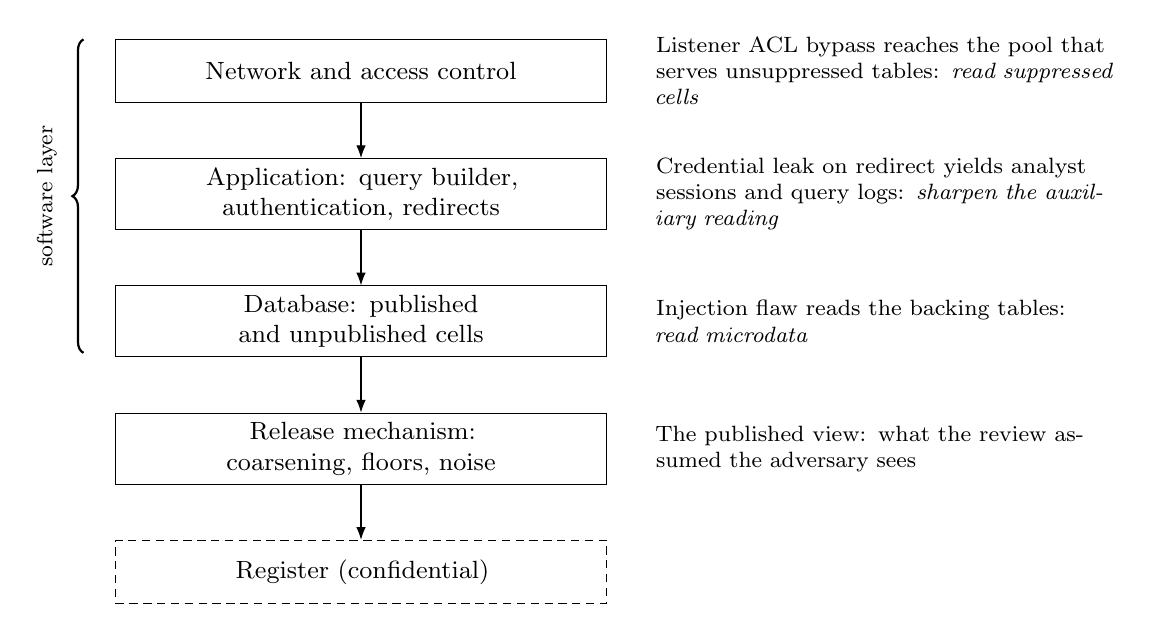
\begin{tikzpicture}[font=\small,
  layer/.style={draw, text width=60mm, minimum height=8mm, align=center},
  note/.style={font=\footnotesize, text width=58mm, align=left, anchor=west}]
\node[layer] (net) {Network and access control};
\node[layer, below=7mm of net] (app) {Application: query builder, authentication, redirects};
\node[layer, below=7mm of app] (db) {Database: published and unpublished cells};
\node[layer, below=7mm of db] (mech) {Release mechanism: coarsening, floors, noise};
\node[layer, below=7mm of mech, densely dashed] (reg) {Register (confidential)};
\node[note] at ($(net.east)+(5mm,0)$) {Listener ACL bypass reaches the pool that serves unsuppressed tables: \emph{read suppressed cells}};
\node[note] at ($(app.east)+(5mm,0)$) {Credential leak on redirect yields analyst sessions and query logs: \emph{sharpen the auxiliary reading}};
\node[note] at ($(db.east)+(5mm,0)$) {Injection flaw reads the backing tables: \emph{read microdata}};
\node[note] at ($(mech.east)+(5mm,0)$) {The published view: what the review assumed the adversary sees};
\draw[decorate, decoration={brace, amplitude=4pt}, thick] ($(db.west)+(-4mm,-4mm)$) -- ($(net.west)+(-4mm,4mm)$) node[midway, left=6pt, rotate=90, anchor=south, font=\footnotesize] {software layer};
\foreach \a/\b in {net/app, app/db, db/mech, mech/reg} {\draw[-{Latex[length=1.6mm]}] (\a) -- (\b);}
\end{tikzpicture}
\caption{Where a software finding sits and what it grants. Each layer above the mechanism can return information the mechanism removed. The dashed box is the register itself, which the method assumes is never served.}
\label{fig:layers}
\end{figure}

We do not need to know which stack an institution runs to make the point; it is enough that any stack has such a list. Table \ref{tab:php} gives the one we use, drawn from the PHP 8.5 changelog for 2026 \citep{phpchangelog}, because PHP is widely deployed in web portals and its advisories are public and dated. The mapping in the last column is to the capability each flaw would grant on a hypothetical PHP-FPM portal in front of a database that holds the unsuppressed tables. Whether a given flaw is exploitable in a given deployment is a finding of the penetration test, not of this table.

\begin{table}[htbp]
\centering\small
\caption{Four PHP advisories of 2026 and the capability each would grant an adversary on a hypothetical PHP-FPM dissemination portal. Severities are the categories used in our plan, not CVSS scores. Source: PHP 8.5 changelog \citep{phpchangelog}.}
\label{tab:php}
\begin{tabular}{llp{52mm}l}
\toprule
Advisory & Release & Flaw & Capability granted \\
\midrule
CVE-2026-91768 & 8.5.11, 24 Sep 2026 & IPv6 ACL bypass in FastCGI \texttt{listen.allowed\_clients} from partial address comparison & read suppressed cells \\
CVE-2026-91766 & 8.5.11, 24 Sep 2026 & HTTP stream wrapper leaks credentials across origins on redirect & sharpen the auxiliary reading \\
CVE-2026-17543 & 8.5.9, 30 Jul 2026 & SQL injection in PGSQL through an \texttt{E'...'} string with a backslash breakout & read microdata \\
CVE-2026-6735 & 8.5.6, 7 May 2026 & Cross-site scripting in the FPM status endpoint & none relevant to disclosure \\
\bottomrule
\end{tabular}
\end{table}

The principle is this. A severity score such as CVSS ranks a flaw by its consequences for the system. A disclosure audit ranks it by its consequences for the people in the register. These are different orderings, and only the second is the statistical office's business. The way to get the second is to treat the flaw as a change in the adversary's information set and measure the declared attack under it.

\section{Penetration testing with the audit}\label{sec:pentest}

\subsection{Capabilities and the adversary view}
\begin{definition}[Capability]
A capability is a named relaxation of the release mechanism as the adversary sees it. The list is closed and declared in code. For the Census release used in the example the list is: read suppressed cells (the floor becomes one); read fine geography (the coarsest geographic width becomes the finest); read fine education (likewise for the education code); sharpen the auxiliary reading (the reading's standard deviation halves, never below the finest declared level); read microdata (all of the above at once).
\end{definition}

\begin{definition}[Finding]
A finding is an identifier, a component, a severity, a status in $\{$confirmed, theoretical, fixed$\}$, a reference, and the set of capabilities it grants.
\end{definition}

\begin{definition}[Adversary view]
For a release $r$ and a set of findings $F$, the adversary view $v(r,F)$ is $r$ with every capability granted by a member of $F$ applied. Capabilities only relax: each component of the view is the minimum of its published value and the value the capability sets.
\end{definition}

\begin{proposition}[Monotone composition]
$v(r,F)$ does not depend on the order of $F$; $v(r,F\cup\{f\})$ is at least as relaxed as $v(r,F)$ in every component; and $v(r,F\cup\{f\})=v(r,F)$ whenever $f$ grants no capability or only capabilities already applied.
\end{proposition}
\begin{proof}
Each component is a minimum over the published value and the values set by the granted capabilities; minimum is commutative, idempotent and non-increasing in the set over which it is taken.
\end{proof}

The proposition is what makes the pooled adversary well defined and what stops a tester from weakening the adversary by listing findings in a convenient order.

\subsection{The protocol}
Algorithm \ref{alg:pentest} gives the protocol. It sits inside the usual testing cycle of planning, discovery, attack and reporting \citep{nist800115}; what it changes is the reporting step, which now produces an audited bound rather than a severity. Its structure is the article's: plan, freeze, measure, certify, with the plan on the ledger before any outcome exists.

\begin{algorithm}[htbp]
\caption{Penetration-test findings as audited adversaries}
\label{alg:pentest}
\KwIn{release $r$ as approved; findings $F$ with statuses; tolerance $\tau$; budget share $\alpha$ for this test cycle; trials $B$; seed; executable attacker $A$; ledger $L$}
\KwOut{a verdict per confirmed finding and for the pooled adversary; the chained record}
$C\gets$ confirmed members of $F$ \tcp*{theoretical and fixed findings are recorded, not audited}
coordinates $\gets[\,(\text{published},\ v(r,\emptyset))\,]$\;
\ForEach{$f\in C$}{append $(f,\ v(r,\{f\}))$}
\If{$|C|>1$}{append $(\text{pooled},\ v(r,C))$}
$\alpha'\gets\alpha/|\text{coordinates}|$\;
$L\gets L\,\Vert\,\text{plan}(r,F,\tau,\alpha,B,\text{seed},\text{coordinates})$ \tcp*{frozen before any draw}
\ForEach{coordinate $(n,v)$ with index $k$}{
  draw $B$ fresh targets from the view $v$ with seed $(\text{seed},k)$\;
  $s\gets A(v,B)$ successes\;
  $u\gets$ exact one-sided upper bound for $s/B$ at level $\alpha'$\;
  $L\gets L\,\Vert\,\text{outcome}(n,s,B,u,\ u\le\tau)$\;
}
verdict $\gets$ \{published within $\tau$; findings whose $u>\tau$; pooled within $\tau$\}\;
$L\gets L\,\Vert\,\text{verdict}$\;
\Return verdict, $L$
\end{algorithm}

Four rules govern its use.
\begin{enumerate}
\item \emph{Status gates the audit.} A theoretical finding is one the tester reports but has not exploited. It is recorded with its capability so the plan shows what would be audited if it were confirmed, and it spends no budget. A fixed finding is kept for the history.
\item \emph{The budget is the programme's.} A test cycle is given a share of the programme's error budget by the tolerance owner, and the cycle splits it equally over its coordinates. A second cycle after remediation is a new share; it does not reuse the first.
\item \emph{The pooled adversary is always audited.} Two findings that each leave the bound below tolerance can fail together; the long form's composition result is the reason, and the worked example shows it.
\item \emph{Remediation is ordered by the bound, not the score.} The finding to fix first is the one whose coordinate breaches by most, then the one whose removal brings the pooled adversary back within tolerance.
\end{enumerate}

\subsection{Worked example}
The example uses the public Census extract that the companion papers use for their public-file experiments \citep{mahomane2026long}: the 29,501-record \texttt{census2000} file, restricted to its first encoded state group (425 records), with the declared linkage attack of the public-file experiment, a matching-key prior and a noisy log-income reading. The release as approved is the coarsest setting in the catalogue: geography width 100, education width 8, minimum cell 10, reading standard deviation 2. The findings are the four advisories of Table \ref{tab:php}, with the two FPM and stream-wrapper flaws marked confirmed, the SQL injection marked theoretical, and the status-page XSS confirmed but granting nothing. Tolerance is 0.2, the cycle's budget share is 0.05, and each coordinate gets 600 fresh trials. Table \ref{tab:pentest} gives the result; the full report and the ledger are in \texttt{artifacts-pentest/} of the code repository \citep{privacyriskcode}, produced by \texttt{scripts/pentest\_demo.py}.

\begin{table}[htbp]
\centering\small
\caption{Penetration-test findings audited as adversary knowledge. Each row is the declared linkage attack run with fresh targets on the release as the named adversary sees it; 600 trials per row, tolerance 0.2, error budget 0.05 split equally over the rows. The upper bound is the exact one-sided binomial bound.}
\label{tab:pentest}
\begin{tabular}{llrrrl}
\toprule
Adversary & View (PUMA, educ., floor, sd) & Successes & Rate & Upper bound & Within \\
\midrule
published & (100, 8, 10, 2) & 60 & 0.100 & 0.132 & yes \\
CVE-2026-91768 & (100, 8, 1, 2) & 222 & 0.370 & 0.417 & no \\
CVE-2026-91766 & (100, 8, 10, 1) & 87 & 0.145 & 0.182 & yes \\
CVE-2026-6735 & (100, 8, 10, 2) & 60 & 0.100 & 0.132 & yes \\
pooled & (100, 8, 1, 1) & 257 & 0.428 & 0.477 & no \\
\bottomrule
\end{tabular}
\end{table}


Four things are visible in Table \ref{tab:pentest}. The release passes as published: 60 successes in 600, upper bound 0.132. The ACL bypass, which lets the adversary read the cells the floor suppressed, takes the bound to 0.417; this release fails under that finding. The credential leak, which halves the reading noise, takes the bound to 0.182: within tolerance on its own. The two together take it to 0.477, worse than either, so a remediation plan that fixed the ACL bypass and left the leak would still have to re-audit, and one that reasoned from the two marginal rows would have been wrong. The XSS finding leaves the view and the bound where they were, as a finding that grants no capability should, and the row is there so that the record shows it was considered. The SQL injection, rated critical, is absent from the table because it was not confirmed; had it been, its row would be the microdata view, and the bound would be the finest-geography risk the companion papers report, far above any tolerance.

The ordering this produces is not the severity ordering. By severity the SQL injection comes first and the XSS third; by measured disclosure risk the ACL bypass comes first, the leak matters only in combination, and the XSS and the unconfirmed injection do not enter.

\section{Deployment}\label{sec:deploy}

\subsection{Architecture}
Figure \ref{fig:architecture} gives the parts and who controls each. The separation follows the five trusted parts of the article's audit-process threat model: the registry that holds budgets and keys, the time source, the target draw, the evaluator, and the record.

\begin{figure}[htbp]
\centering
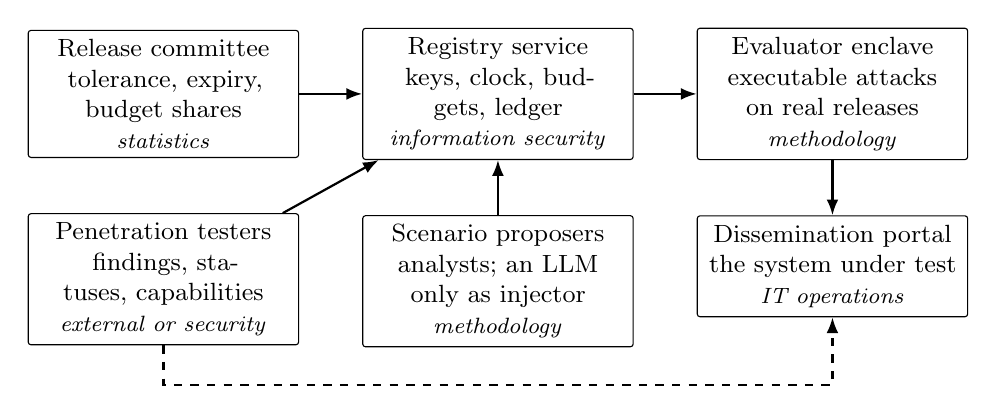
\begin{tikzpicture}[font=\small, node distance=7mm and 8mm,
  part/.style={draw, rounded corners=1pt, minimum height=11mm, text width=32mm, align=center},
  arr/.style={-{Latex[length=2mm]}, thick}]
\node[part] (committee) {Release committee\\tolerance, expiry, budget shares\\{\footnotesize\itshape statistics}};
\node[part, right=of committee] (registry) {Registry service\\keys, clock, budgets, ledger\\{\footnotesize\itshape information security}};
\node[part, right=of registry] (evaluator) {Evaluator enclave\\executable attacks on real releases\\{\footnotesize\itshape methodology}};
\node[part, below=of committee] (redteam) {Penetration testers\\findings, statuses, capabilities\\{\footnotesize\itshape external or security}};
\node[part, below=of registry] (proposer) {Scenario proposers\\analysts; an LLM only as injector\\{\footnotesize\itshape methodology}};
\node[part, below=of evaluator] (portal) {Dissemination portal\\the system under test\\{\footnotesize\itshape IT operations}};
\draw[arr] (committee) -- (registry); \draw[arr] (registry) -- (evaluator);
\draw[arr] (redteam) -- (registry); \draw[arr] (proposer) -- (registry);
\draw[arr] (evaluator) -- (portal);
\draw[arr, dashed] (redteam.south) -- ++(0,-5mm) -| (portal.south);
\end{tikzpicture}
\caption{Deployment architecture. Every declaration, plan and outcome passes through the registry, which alone holds the signing key, the time source and the programme budgets. Testers probe the portal (dashed) and declare findings to the registry; they never run the evaluator. Proposers, human or machine, only propose: the closed-network rule of the companion papers.}
\label{fig:architecture}
\end{figure}

Three design choices follow from the article's measured attacks on the audit process. The registry is a separate service with its own storage and key, because a ledger the operator can rewrite proves nothing. Target seeds are derived from a commitment the operator makes at registration and a public randomness beacon named for a later round, because an operator who can grind seeds certifies an unsafe attack in most runs. And bets, where the anytime-valid procedure is used, are committed before each draw. The companion code implements each of these as a library; the deployment turns them into a service.

\subsection{Roles}
The tolerance owner is the head of the statistical function, because the tolerance is a judgement about harm to reporting institutions and about the value of the product. The registry is operated by the information-security function, not by statistics, so that the people who want a release to pass do not hold the key that records whether it did. The evaluator is run by methodology inside the enclave that already holds the confidential data. Penetration testers are external or report to security; they declare findings and statuses and never touch the evaluator. Scenario proposers are analysts, and a language model may be among them only under the closed-network rule: it proposes, a named reviewer approves, the evaluator measures, and nothing it writes reaches the record as evidence.

\subsection{Phases}
\begin{description}
\item[Shadow run.] One programme, past releases. Declare the adversaries, run the attacker, write the ledger, gate nothing. The output is a calibrated view of what the current rules have been releasing and the compute the tolerance will cost. For the banking statistics this is the quarterly series over several years and the two views.
\item[Gated run.] The committee sets the tolerance and the budget, the registry goes live, and new releases of that programme pass through the gate. A failed audit is a decision record, not an emergency: the long form's protocol says what the committee does with it.
\item[Security integration.] The penetration-testing cycle of Section \ref{sec:pentest} joins the gated programme with its own budget share. Findings from routine testing and from advisories such as those in Table \ref{tab:php} are declared as they arrive, and the ordering they produce feeds remediation.
\item[Extension.] A second programme, then the Hub, where the insider coordinate and the access-control mechanism make the audit different in kind: the view is not a coarsened table but a set of accounts, and the capability list is written for that.
\end{description}

\section{Limits and what is not claimed}\label{sec:limits}
The mapping of Table \ref{tab:programmes} rests on public descriptions; the BIS's internal mechanisms, stack and controls are not known to us and nothing here describes them. The PHP advisories are real and the capability mapping is plausible for the stack we describe, but we have not exploited any of them, and the example assumes exploitability; in a deployment that assumption is the tester's finding, recorded with a status. The worked example is one public file, one attack, one state group, and the bounds are conditional on that file and on simulated auxiliary readings; they are not population risk. The capability list is closed by design, which means a finding whose effect is not on the list cannot be audited until the list is extended and the extension is declared; that is a feature, since an undeclared relaxation is exactly what the method refuses to reason about, but it is also work. The registry service is specified, not built; the companion code gives the library. And a measured attack on a relaxed view says what the declared adversary achieves; it does not say that no other adversary achieves more.

\section{Conclusion}
The method of the companion papers asks an institution to say who the adversary is, to measure what that adversary achieves, to spend one error budget on the answer, and to keep a record it cannot quietly rewrite. This paper shows that the BIS's programmes have the features that make those asks worth meeting, lays out the roles and phases for meeting them, and adds one rule: a software flaw is a change in what the adversary knows, so a penetration test is a source of adversaries, and its findings should be audited with the same attacker, at the same budget, on the same ledger as everything else. Done that way, security testing and disclosure control stop being two reports and become one.

\subsection*{Data and code}
The worked example runs from \texttt{scripts/pentest\_demo.py} in the companion repository \citep{privacyriskcode}; its report, ledger and table are committed under \texttt{artifacts-pentest/} and \texttt{paper/generated/}. The red-team harness is \texttt{privacy\_risk.redteam}, with tests. No confidential data were used.

\begin{thebibliography}{9}\small
\bibitem[BIS(2026)]{bisstats}
Bank for International Settlements (2026): \emph{BIS statistics}, \url{https://www.bis.org/statistics/index.htm}, accessed 23 October 2026.
\bibitem[Mahomane(2026a)]{mahomane2026long}
Mahomane, R R M (2026a): ``Governing privacy risk across repeated statistical releases: probability models, programme tolerances and accountable decisions'', author manuscript, long form for the Irving Fisher Committee, with online appendix.
\bibitem[Mahomane(2026b)]{mahomane2026adaptive}
Mahomane, R R M (2026b): ``Adaptive certification of attack-conditional disclosure risk across release programmes'', author manuscript.
\bibitem[Mahomane(2026c)]{privacyriskcode}
Mahomane, R R M (2026c): \emph{Privacy Risk Thresholds: reproducible research pipeline}, software, \url{https://github.com/Nube1/privacy-risk-thresholds}.
\bibitem[PHP Group(2026)]{phpchangelog}
The PHP Group (2026): \emph{PHP 8 ChangeLog}, \url{https://www.php.net/ChangeLog-8.php}, releases 8.5.6 to 8.5.12, accessed 23 October 2026.
\bibitem[Scarfone et al.(2008)]{nist800115}
Scarfone, K, M Souppaya, A Cody and A Orebaugh (2008): \emph{Technical guide to information security testing and assessment}, NIST Special Publication 800-115, National Institute of Standards and Technology.
\end{thebibliography}
\end{document}
